%--------------------------------------------
%	PACKAGES AND DOCUMENT CONFIGURATIONS
%--------------------------------------------

\documentclass[11pt]{article}

\usepackage{fancyhdr}
\usepackage{pgfplots}
\usepackage{gensymb}
\usepackage[ampersand]{easylist}
\usepackage[a4paper, total={8.5in, 11in}, margin = 1.0in]{geometry}

\usepackage[version=3]{mhchem} % Package for chemical equations
\usepackage{siunitx} % The \SI{}{} and \si{} command for SI units
\usepackage{graphicx, epstopdf} % Required for the inclusion of images
\usepackage{natbib} % Required to change bibliography style to APA
\usepackage{amsmath} % Required for some math elements
\usepackage[framed,numbered]{matlab-prettifier}

\setlength\parindent{0pt} % Removes all indentation from paragraphs

\renewcommand{\labelenumi}{\alph{enumi}.} % Make numbering in the enumerate environment by letter rather than number 

\setcitestyle{square}

%----------------------------------------------
%	DOCUMENT INFORMATION
%----------------------------------------------
\title{ \textbf{Laboratory 2: Sensor Interfacing}}

\author{
	\begin{tabular}{c}
	    Whitney Chu\\
		Adesh Kadambi\\
		Jasen Devasagayam\\
		Chisomeje Umeonyido\\\\
	\end{tabular}
	
}

\date{}

\begin{document}
\begin{titlepage}
    \centering
    \maketitle
    \thispagestyle{empty}
\end{titlepage}

\newpage
\renewcommand{\abstractname}{Executive Summary}
\begin{abstract}
\thispagestyle{empty}
This lab explored the use of various sensors to collect data in the physical environment to allow a user to interpret it intuitively. The first experiment took distance measurements using an ultrasonic sensor (HC-SR04). The second experiment measured atmospheric pressure, temperature, humidity, and sea level (with respect to sea level) with a BME280 Breakout Board. The microcontroller used to process all the collected data is the RedBear Duo Microcontroller.\\

The following report contains the setup used for the lab, including the ultrasonic sensor, breakout board, as well as post-processing of the data. The methodology is then followed by the static response of the ultrasonic sensor as well as a dynamic response, showing responses with a time aspect. The next section includes a calibration curve of the temperature sensor of the BME280, and dynamic responses using a hot and cold cup. Both of the static datasets contain error bars which were analyzed, as well as time constants for the temperature sensor. \\

An analysis was done on the errors presented in the lab, as there were many areas where errors did occur. Possible reasons for error were mentioned throughout the report. The lab experiments consisted of many defective and error-prone components which resulted in unexpected results. In addition, the defective instruments presented some problems that made data acquisition difficult. These problems had occurred in microcontrollers as well as the sensors themselves.\\

The report is then concluded by presenting future recommendations based on errors and difficulties of performing these experiments. The appendix of this report also presents the source code used to process the data and display the results. 
\end{abstract}

\pagebreak

\thispagestyle{empty}
\tableofcontents
\listoffigures
%\listoftables
%\lstlistoflistings
\newpage

\pagenumbering{arabic}

\section{Introduction}

In instrumentation, sensors are needed to acquire information on physical quantities and conditions, and their change over time. In medical instrumentation, sensors acquire information on biological parameters such as heart rate, internal blood pressure, neural electrical activity, and body temperature. The purpose of this lab was to introduce students to sensor
 interfacing, which included data acquisition of the sensors and control of the sensors using a microcontroller. The sensors used in this lab were an HC-SR04 ultra-sonic distance sensor and a SparkFun\textsuperscript{TM} BME280 Temperature Humidity Sensor Module. Originally, a \textit{Parallax Ping)))\textsuperscript{TM}}  Ultrasonic sensor was used, however the device was defective so an HC-SR04 sensor was used. The sensors were interfaced using a RedBear Duo \textsuperscript{TM} microcontroller. The HC-SRO4 sensor was used to measure distance at various points, and the BME280 sensor was used to gather the temperature and humidity of the room at different heights, and conditions. The accuracy of the sensors in addition to their dynamic response were evaluated in this lab. \\

Each sensor operates by taking advantage of a physical principle, in which a property is measured then converted to a corresponding electrical signal, either a voltage or a current, to be interpreted by a control unit. The ultrasonic sensor operates by detecting acoustic waves, and the BME280 detects temperature and humidity through a change in material properties at different conditions. \\

\subsection{Ultrasonic Sensor}

The Ultrasonic Sensor consists of an ultrasonic receiver, and ultrasonic transmitter and a control circuit \cite{HTM,Spark}. Ultrasound at a frequency of 40,000 Hz is emitted by the transmitter. The sound wave is reflected by objects near the sensor, and the reflected wave is then detected by the receiver, which measures the time that was taken for the wave to be detected \cite{HTM}. At a known speed of sound, the time for the signal to return can be used to find the distance from the sensor to an object. The range of an ultrasonic sensor is generally around 5 metres\cite{Prac}, however the range of the HC-SRO4 is 4m according to the datasheet. The distance at which the sensors detect an object is also heavily dependant on the geometry of the body, such that curved surfaces and unsmooth areas can reflect the transmitted wave in a different direction \cite{Prac}. Properties that affect the speed of sound such as air pressure and temperature will also affect the readings of the sensor. At a constant pressure of 1atm, the speed of sound, $V_{sound}$, with respect to temperature, T, can be approximated by the following formula\cite{Hyper}:

\begin{equation}
    V_{sound} = 331.1 m/s + 0.6T
\end{equation}    

The limitations of an ultrasonic sensor still allow for it to be suitable in applications where an approximate distance is needed, hobbyist robotics, and motion detection. \\

\subsection{BME280 Breakout Board}

The sensor used to measure temperature, humidity, and pressure is the BME280 Breakout Board. This sensor also measured altitude changes, from sea level. It is commonly interfaced with a RedBear or an Arduino. The sensor contains two communication protocols; one is the Inter-Integrated Circuit (I\textsuperscript{2}C) protocol, and the other is the Serial Peripheral Interface (SPI) protocol. Both I\textsuperscript{2}C and SPI protocols are used for short-distance communications and they both exchange information using two signal wires.\\

The main difference between the two protocols is the number of connections needed to allow the communication to occur \cite{I2C}. The SPI protocol requires four wires to connect each device to the controller. This can make it difficult to interface multiple devices, as the set up may get complicated and messy. However, SPI is useful to collect data at a high rate with multiple inputs, sampling at rates above 10MHz at times. The I\textsuperscript{2}C protocol requires only two lines and it can support multiple devices (up to 1008). This makes for an easy and clean wiring job. This protocol normally samples at rates from 100kHz to 400kHz. However, according to the datasheet, this sensor can sample up to 10MHz in SPI, and up to 3.4 MHz in I\textsuperscript{2}C \cite{BME}. For this lab, the I\textsuperscript{2}C protocol was used. \\
	
The supply voltage on the BME sensor requires 3.3V, so a logic level converter was not needed to shift from a 5V supply to 3.3V \cite{BME}. There is no processing of the output data required, as the system displays the values directly, if interfaced properly. The humidity sensor requires a supply current of $1.8\mu$A - $2.8\mu$A and displays values from 0 - 100\% relative humidity, with a resolution of 0.008\%. The pressure sensor requires a supply current of $2.8\mu$A to $4.8\mu$A and can resolve pressure values from 300hPa to 1100hPa at a resolution of 0.18Pa. The temperature sensor operates at a range of -40\textdegree C to 85\textdegree C and requires a supply current of $1.0\mu$A. The resolution of the temperature sensor is 0.01\textdegree C \cite{BME}. The block diagram for the BME280 can be seen below in Figure \ref{fig:block}.\\

\begin{figure}[ht]
    \centering
    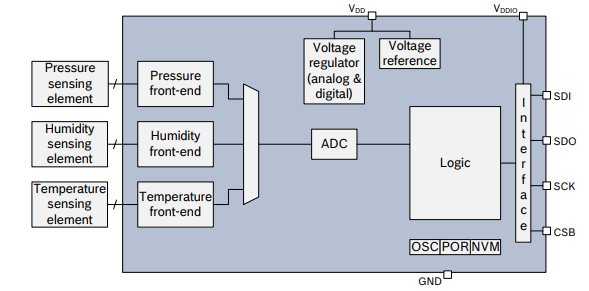
\includegraphics[width=0.8\textwidth]{pics/block.PNG}
    \caption{Block Diagram of BME280}
    \label{fig:block}
\end{figure}

\subsection{RedBear Duo Microcontroller}

The RedBear Duo is a microcontroller that allows for the sensors to be interfaced with a control unit so that the data that is acquired may be readily analyzed, converted to a different form, and displayed. A micro controller is a device consisting of a central processing unit (CPU), memory for data storage, I/O ports for interfacing with other components, interrupts which break the instruction sequence in a program, and Analog to Digital Converters (ADC) and Digital to Analog Converters (DAC) \cite{Hub}. They are used to control other components in electrical or mechatronic systems. Micro controllers have the advantage of having all essential components of a computer system integrated onto a single chip, which also reduced the area that components consume. All their ports are programmable which allows for ease of control of external parts.\\ 

The RedBear Duo has these features. The RedBear uses the ARM cortex M3 chip as its CPU and features 18 I/O ports. Some of these ports allow for specific communication protocols to be implemented when interfacing with sensors, in which the micro controller is called the master device and the sensors are called the slave devices \cite{Prac}. In this lab, the integr-integrated communication or I\textsuperscript{2}C, and Serial Peripheral interfacing (SPI) were the protocols that could have been used for the sensors. I\textsuperscript{2}C uses two wires to communicate; a Serial Data Line (SDA) over which data is transferred to a slave device, and a Serial Clock Line (SCL) which sets the timing of the data transfer \cite{Prac}. SPI uses four lines of communication; a MISO line which sends information from the slave to the master device, a MOSI line which sends data from the master to the slave device, a slave select line which selects the device to communicate with, and a clock line that controls the timing of communication \cite{Prac}. The communication protocols allow for control of the sensor and data acquisition.\\

The lab served to introduce students to sensor integration and control through use of a RedBear Duo, and Ultrasonic sensor, and a Temperature and Humidity Sensor. The evaluation and analysis of the data gathered by each sensor through the dynamic response and the accuracy were assessed. \\

\section{Methodology}

The main goal of this lab was to collect data from the Ultrasonic Distance Sensor and the Breakout sensor which can be seen below in Figures \ref{fig:breakout} and \ref{fig:ultasound}.

\begin{figure}[ht]
    \centering
    \begin{minipage}{0.45\textwidth}
        \centering
        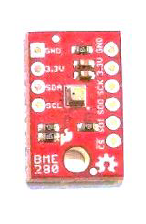
\includegraphics[width=0.42\textwidth]{pics/breakout_sensor.PNG}
        \caption{Breakout Sensor}
        \label{fig:breakout}
    \end{minipage}\hfill
    \begin{minipage}{0.45\textwidth}
        \centering
        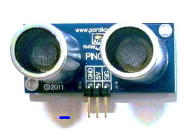
\includegraphics[width=0.9\textwidth]{pics/ultrasound.PNG}
        \caption{Ultrasonic Distance Sensor}
        \label{fig:ultasound}
    \end{minipage}
\end{figure}

\subsection{Initial Set-Up}

The initial set-up included connecting everything correctly and testing the different components used in the lab to ensure they were working properly. The first step was to set up the RedBear Duo micro-controller. In order to do this, Arduino was opened up on the desktop and set up to support the RedBear Duo and the package was installed on the board manager. The Redbear was connected to the breadboard as seen in Figures \ref{fig:sch_sonic} and \ref{fig:sch_temp}.\\

The USB cable was connected to the computer and the microUSB port on the RedBear. The Redbear was put into DFU mode by holding down both the RESET and SETUP button and then releasing the RESET button while still holding down the SETUP button until the LED light started to blink yellow. The proper board and serial port were chosen and the bootloader was  burned to the RedBear Duo. An example code was uploaded and run to ensure the components were working.\\

\begin{figure}[!ht]
    \centering
    \begin{minipage}{0.45\textwidth}
        \centering
        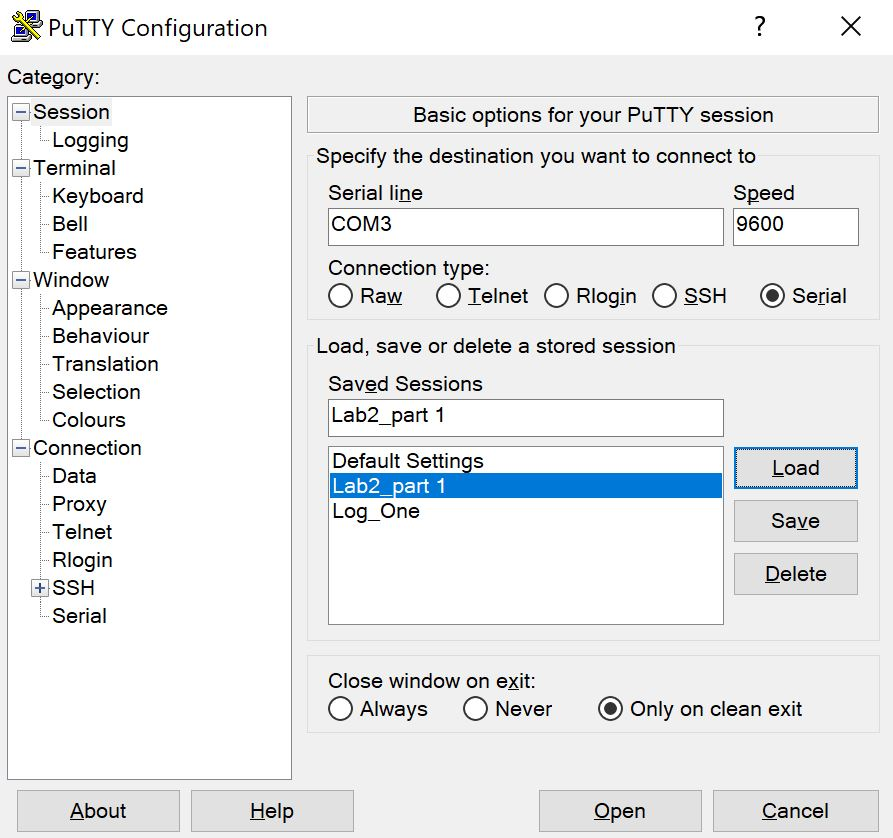
\includegraphics[width=0.85\textwidth]{pics/Putty_shot_1.JPG}
        \caption{PuTTY session settings.}
        \label{fig:puttys1}
    \end{minipage}\hfill
    \begin{minipage}{0.5\textwidth}
        \centering
        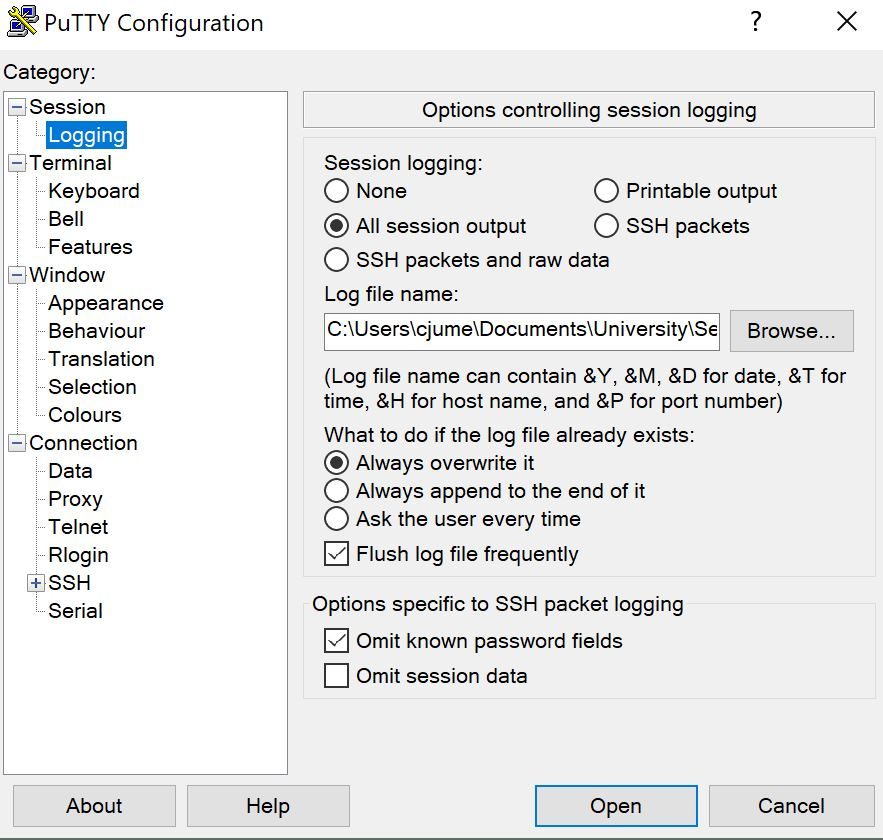
\includegraphics[width=0.8\textwidth]{pics/Putty_shot_2.JPG}
        \caption{PuTTY logging settings.}
        \label{fig:puttys2}
    \end{minipage}
\end{figure}

The PuTTY software was used to gather the data from the serial monitor. As seen in Figure \ref{fig:puttys1}, the sessions section of the PuTTY is displayed and the connection type is set to serial. The speed of communciation is set to 9600, and the serial line was set to {\fontfamily{qcr}\selectfont COM4}. In Figure \ref{fig:puttys2}, the logging section of PuTTY is displayed and a textfile is added to the PuTTY interface. The system has been configured to overwrite the text file every time. A new textfile was added to PuTTY before the begining of ta trial so that the data may be recorded. 

\subsection{Ultrasonic Distance Sensor}

The first part of the lab used the ultrasonic distance sensor. The code from Appendix A in the Lab 2 - Sensor Interfacing lab manual was copied and pasted into Arduino and functions for the conversion of data collected were written and named {\fontfamily{qcr}\selectfont MetresToIn} and {\fontfamily{qcr}\selectfont MetresToCm}. The ultrasonic distance sensor was connected to the breadboard and wires were also used to connect the RedBear to the sensor following the schematic below in Figures \ref{fig:schematic} and \ref{fig:sch_sonic}.\\


\begin{figure}[!ht]
    \centering
    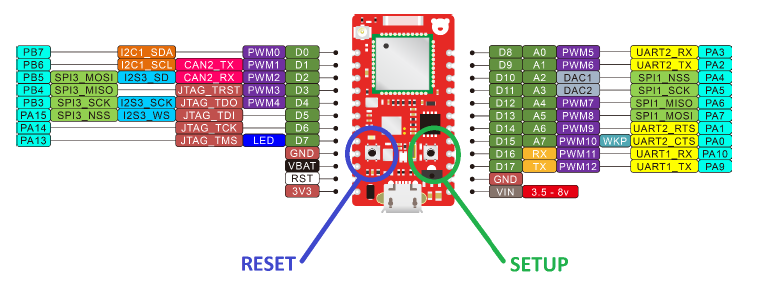
\includegraphics[width=0.90\textwidth]{pics/schematic.PNG}
    \caption{Schematic of the Duo Micro-controller}
    \label{fig:schematic}
\end{figure}

\begin{figure}[!ht]
    \centering
    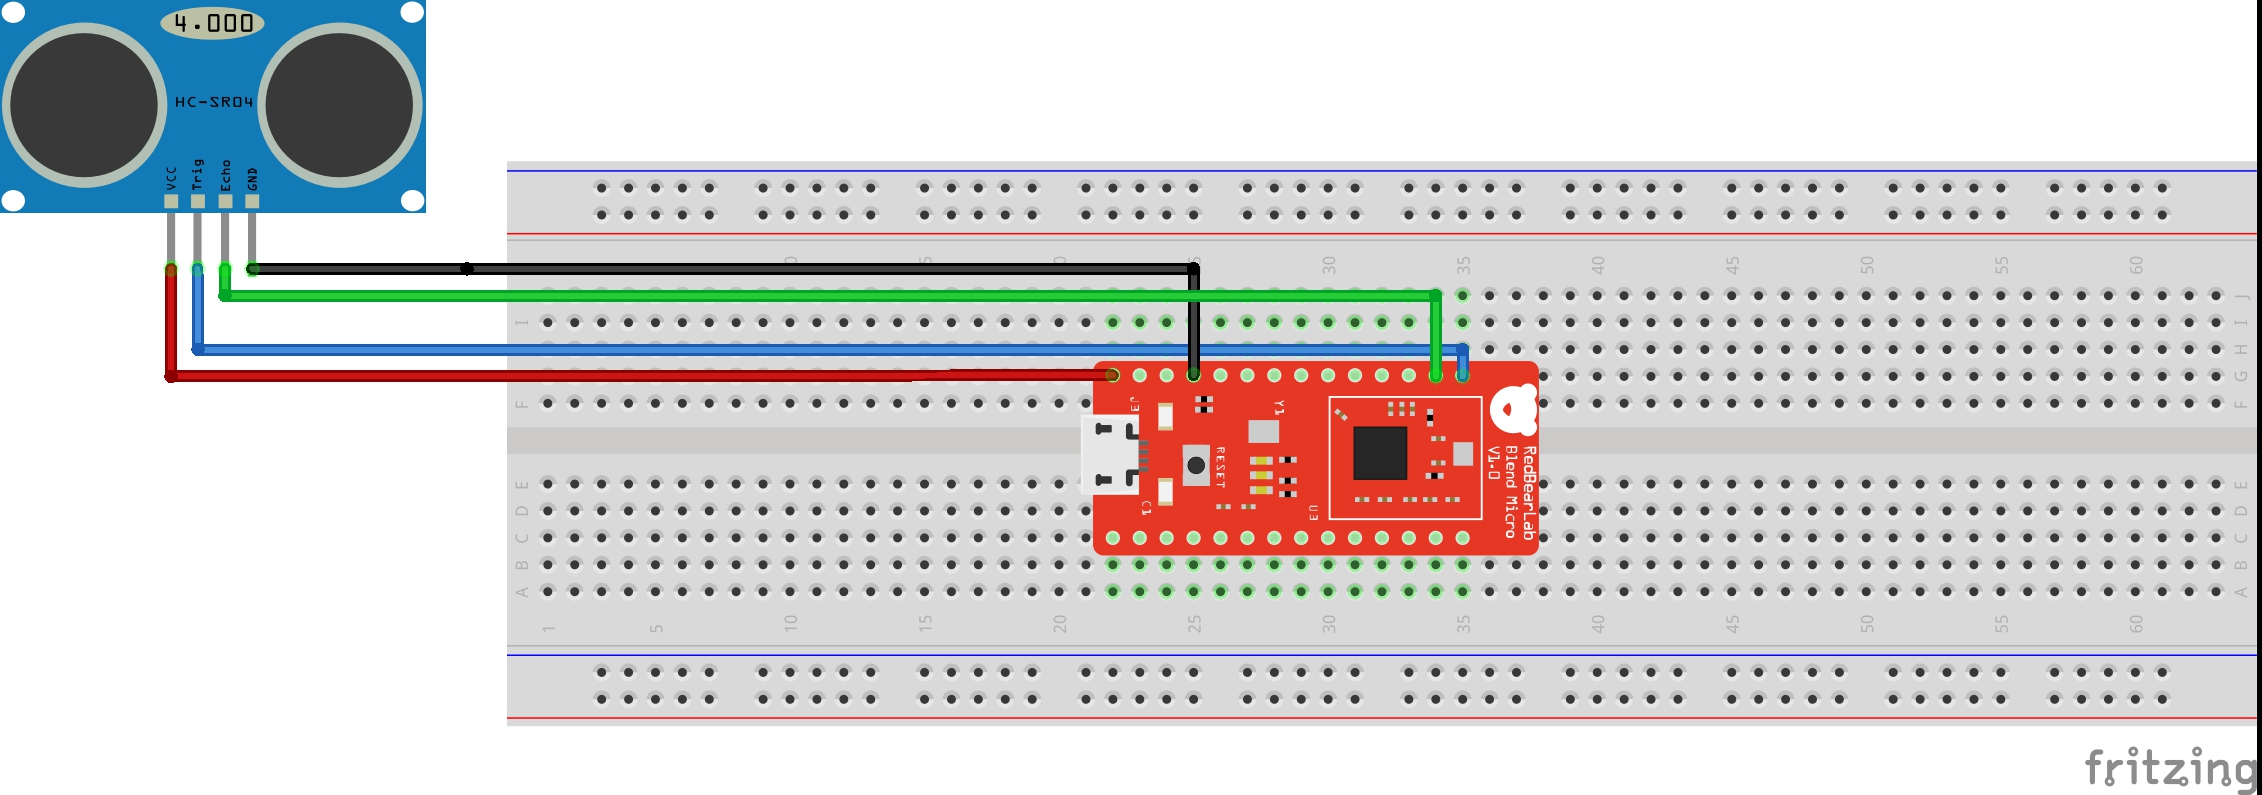
\includegraphics[width=0.8\textwidth]{pics/UltrasonicSensor.jpg}
    \caption{Schematic of Ultrasonic Sensor}
    \label{fig:sch_sonic}
\end{figure}

The code from Appendix A in the ``Lab 2 - Sensor Interfacing" lab manual allowed us to obtain data values using the PuTTY software. A measuring tape was taped to the ground starting at the sensor and extending outwards in order to compare the known distances and distances outputted by the ultrasonic Sensor. Multiple distances were tested and around 20 measurements were taken, 5 seconds apart at each distance.\\

\subsection{BME280: Breakout Board}

The second part of the lab used the Breakout Board to measure temperature, humidity, and pressure. One end of the jumper wires were soldered to the breakout sensor at pins {\fontfamily{qcr}\selectfont GND, 3.3V, SDA,} and {\fontfamily{qcr}\selectfont SCL}, while the other end was connected to the breadboard. To interface the BME280, the circuit was reconnected to match the schematic shown in Figures \ref{fig:schematic} and \ref{fig:sch_temp}.\\ 

\begin{figure}[ht]
    \centering
    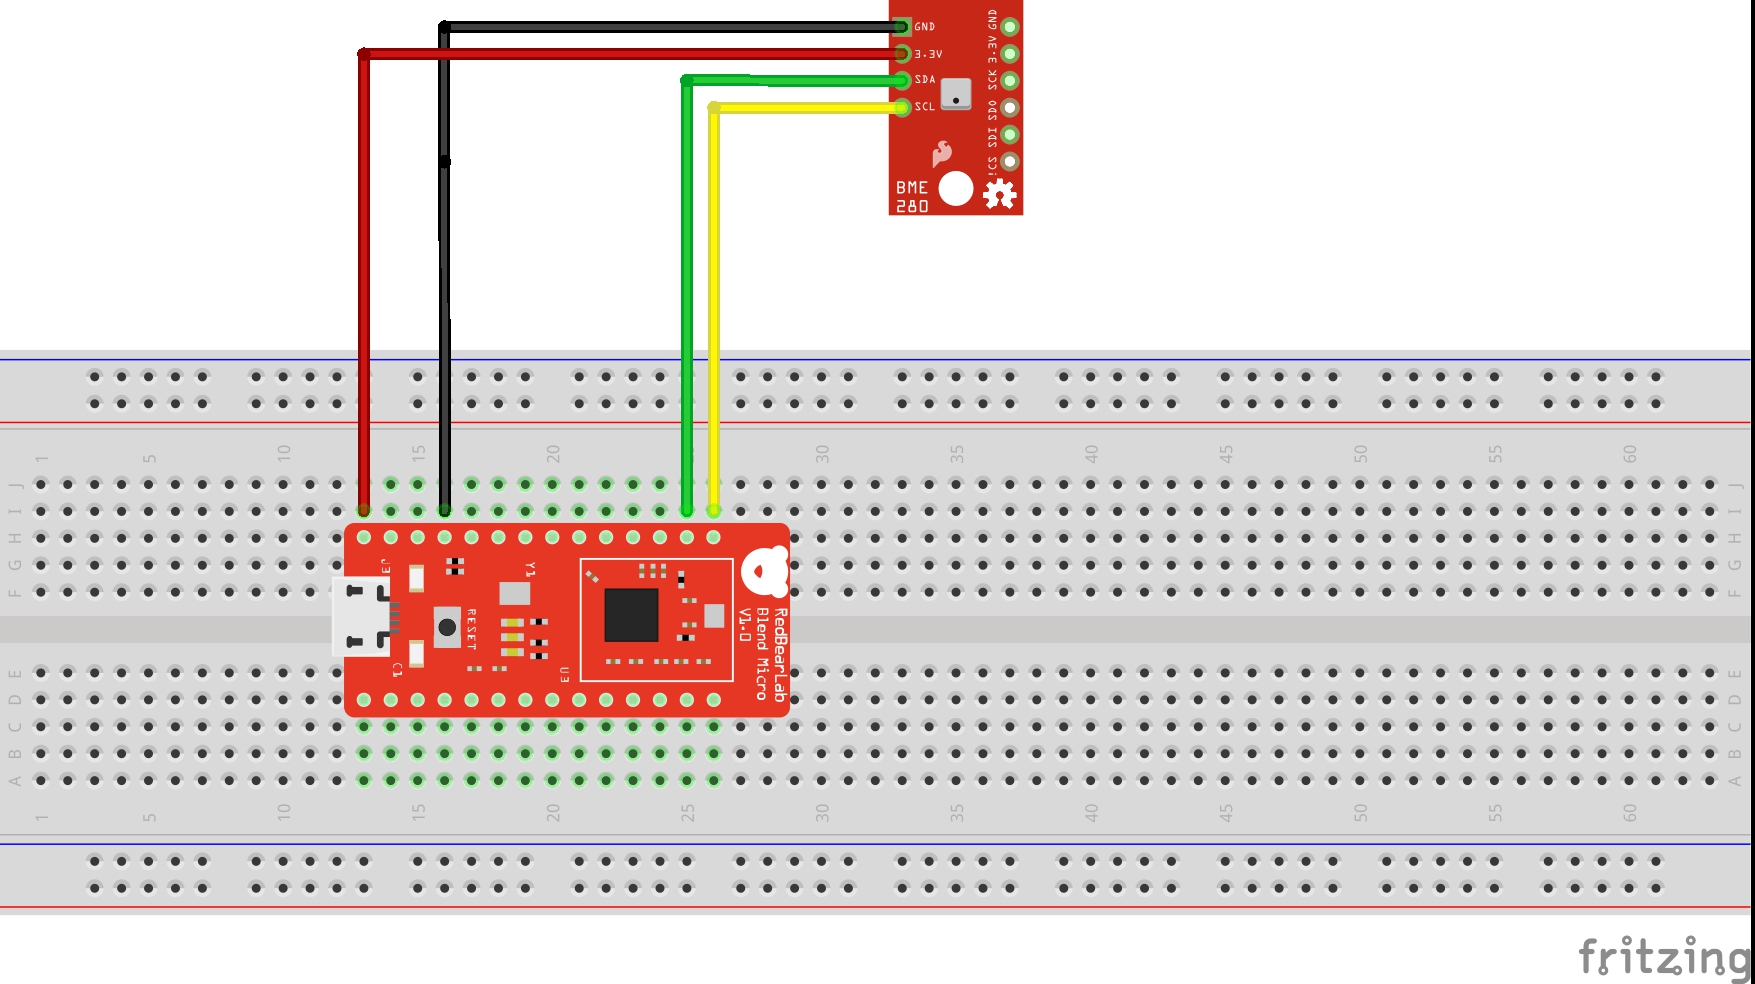
\includegraphics[width=0.8\textwidth]{pics/BME280Sensor.jpg}
    \caption{Schematic of BME:280 Sensor}
    \label{fig:sch_temp}
\end{figure}

``SparkFun" was installed into the Arduino library and the example code was used to record the data. Several measurements were taken at six different heat and altitude locations with each measurement at least 5 seconds apart. The six different locations were: (1) an open desk surface, (2) above a cup with room temperature water, (3) above a cup with cold water, (4) above a cup with hot water, (5) high altitude, and (6) low altitude. The BME sensor is not waterproof, so it had to be held above the water to prevent damage to the sensor.  

\subsection{Signal Processing}
All signal processing was performed using MATLAB (MathWorks Inc., Massachusetts, USA). To produce the calibration curves, all the PuTTY output files were imported into MATLAB using the built-in {\fontfamily{qcr}\selectfont uiimport} and {\fontfamily{qcr}\selectfont importdata} functions. The standard deviation and mean were taken for the data output from both the PING))) ultrasonic sensor (distance) and BME280 Breakout Board (temperature and elevation). Linear regression was then performed by determining {\fontfamily{qcr}\selectfont b0} and {\fontfamily{qcr}\selectfont b1} coefficient values and plotting the line of best fit for all three cases using the function displayed in Listing 5. The built-in function, {\fontfamily{qcr}\selectfont errorbar}, was used to plot error bars to each point. The code for distance calibration is seen in Listing 3 and elevation calibration is seen in Listing 4.\\

\section{Results}
\subsection{Ultrasonic Sensor}
% Calibration plots: dist vs. dist, elevation vs. elevation, temp vs. temp, accuracy/precision
% Dynamic Responses: dist vs. time, temp vs. time, hysteresis, 1st order time constant

\begin{figure}[!ht]
\centering
\makebox[0pt]{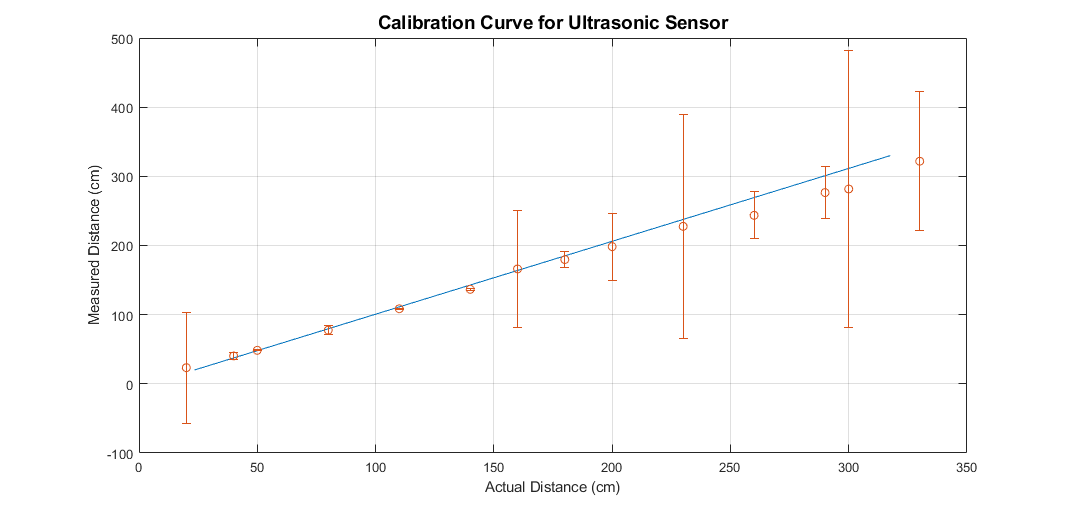
\includegraphics[height=3.2in]{pics/sonic_calibration.png}}
\caption{Calibration curve for ultrasonic sensor.}
\label{fig:sonic_cal}
\end{figure}

The calibration curve for the ultrasonic sensor can be seen in Figure \ref{fig:sonic_cal}. The blue line represents the line of best fit created from the regression. The $R^{2}$ value of the regression was 0.974, indicating a very strong linear relationship between the actual and measured distance of the sensor. Very high standard deviations can be observed in the data after exceeding 200cm. From the calibration curve it can be seen that the linear region of the sensor resides between 30cm and 150cm.\\

\begin{figure}[!ht]
    \centering
    \begin{minipage}{0.5\textwidth}
        \centering
        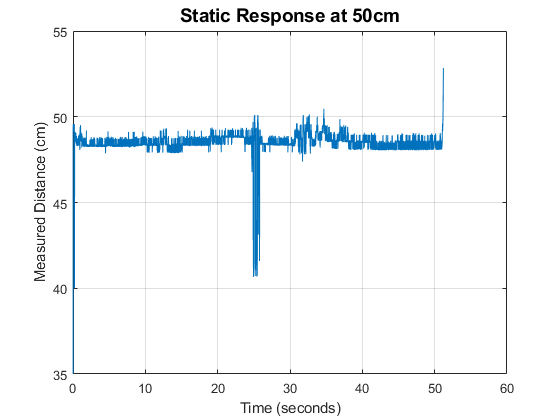
\includegraphics[width=1.0\textwidth]{pics/50static.png}
        \caption{Static response at 50cm.}
        \label{fig:50static}
    \end{minipage}\hfill
    \begin{minipage}{0.5\textwidth}
        \centering
        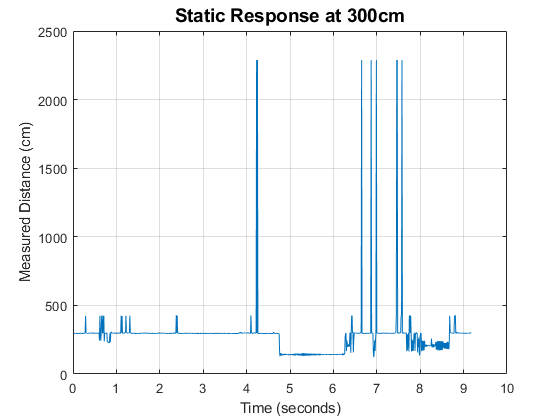
\includegraphics[width=1.0\textwidth]{pics/300static.png}
        \caption{Static response at 300cm.}
        \label{fig:300static}
    \end{minipage}
\end{figure}

From the static response plots in Figures \ref{fig:50static} and \ref{fig:300static}, it can be seen that a distance that is kept within the linear region is fairly steady whereas the static response for 300cm that is both outside the linear region and the upper limit of the ultrasonic sensor has various fluctuations that result in spikes of over 2000cm.\\

Note: Static responses were used for comparison since step responses were not taken.

\pagebreak
\subsection{BME Sensor}

\begin{figure}[!ht]
\centering
\makebox[0pt]{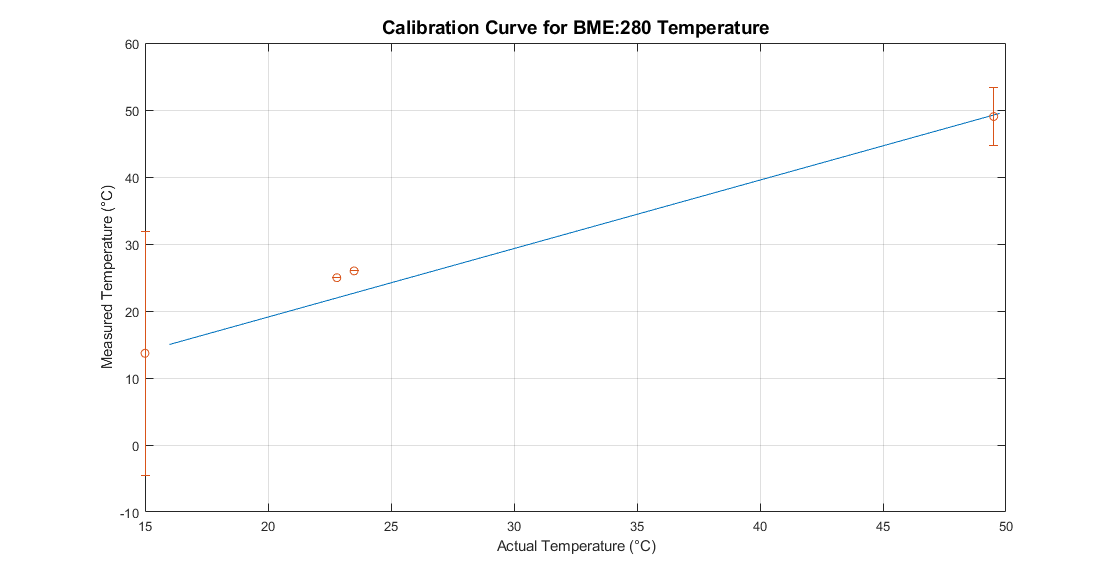
\includegraphics[height=3.2in]{pics/temp_cal.png}}
\caption{Calibration curve for BME280 temperature.}
\label{fig:temp_cal}
\end{figure}

The calibration curve for the temperatures recorded by the BME280 breakout board can be seen in Figure \ref{fig:temp_cal}. With an $R^{2}$ value of 0.9842, the temperature recorded by the sensor is fairly accurate. It is important to note that error bars are very low except for the cold cup at 15\textdegree C. This is due to experimental error that caused temperature fluctuations in the cup while positioning it above the ice instead of in the ice.\\

The percentage error of the sensor was calculated using the equation below where $n_{exp}$ is the sensor measurement and $n_{th}$ is the thermometer measurement:

\begin{equation}
    \%_{err} = \frac{n_{exp} - n_{th}}{n_{th}}*100
\end{equation}

This percentage error is a method for validating the precision of the sensor against the standard, in our case, the thermometer. The percentage error can be seen in Table \ref{table:per_err} below.

	\begin{table}[ht]
    \caption{Percentage error for BME280 at various temperatures.}
	\vspace{3mm}
	\centering
	\begin{tabular}{cccc}
	\hline
		Measured Temperature & Actual Temperature & Difference & Percentage Error\\
	\hline
		13.7\textdegree C & 15.0\textdegree C & -1.3\textdegree C & 8.67\%\\
		24.9\textdegree C & 22.8\textdegree C & 2.1\textdegree C & 9.21\%\\
		26.0\textdegree C  & 23.5\textdegree C & 2.5\textdegree C & 10.64\%\\
		49.0\textdegree C  & 49.5\textdegree C & -0.5\textdegree C & 1.01\%\\
	\hline
	\end{tabular}
	\label{table:per_err}
	\end{table}

\begin{figure}[!ht]
\centering
\makebox[0pt]{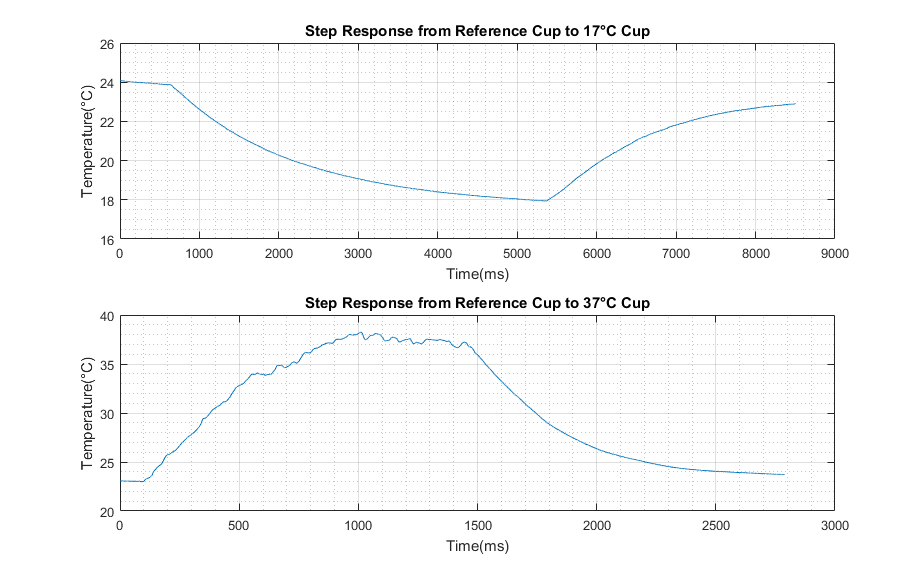
\includegraphics[width=1.2\linewidth]{pics/Subplots.png}}
\caption{Step Responses of BME280 Temperature Sensor}
\label{fig:Subplots}
\end{figure}

To observe the dynamic response of the BME280 sensor, step responses for 17\textdegree C and 37\textdegree C were taken as seen in Figure \ref{fig:Subplots}. These responses were taken from the provided data on Courselink. The time constant, $\tau$, was calculated to determine the responsiveness of the BME280 using Equation 3 below for an increasing step response and Equation 4 for a decreasing step response. The total response time of the BME280 is represented by approximately $5\tau$ which corresponds to 99.3\% of the total response. As a result, this value can be used to determine steady state when using the sensor for future readings. The calculated time constants are shown in Table \ref{table:tau}.\\

\begin{equation}
    T(t) = T_{o}(1-e^{-t/\tau})
    \vspace{3mm}
\end{equation}
\begin{equation}
    T(t) = T_{o}e^{-t/\tau}
    \vspace{3mm}
\end{equation}
\pagebreak

	\begin{table}[!ht]
    \caption{Time constants for step responses.}
	\vspace{3mm}
	\centering
	\begin{tabular}{ccc}
	\hline
		Cup Temperature & $\tau$ (seconds) & $5\tau$ (seconds)\\
	\hline
		17\textdegree C & 1.48 & 7.40\\
		37\textdegree C & 0.70 & 3.50\\
	\hline
	\end{tabular}
	\label{table:tau}
	\end{table}

The calibration curve for the elevation recorded by the BME280 breakout board can be seen in Figure \ref{fig:ela_cal}. With an $R^{2}$ value of 0.9925, the elevation recorded by the sensor demonstrates a very strong linear relationship.\\

\begin{figure}[ht]
\centering
\makebox[0pt]{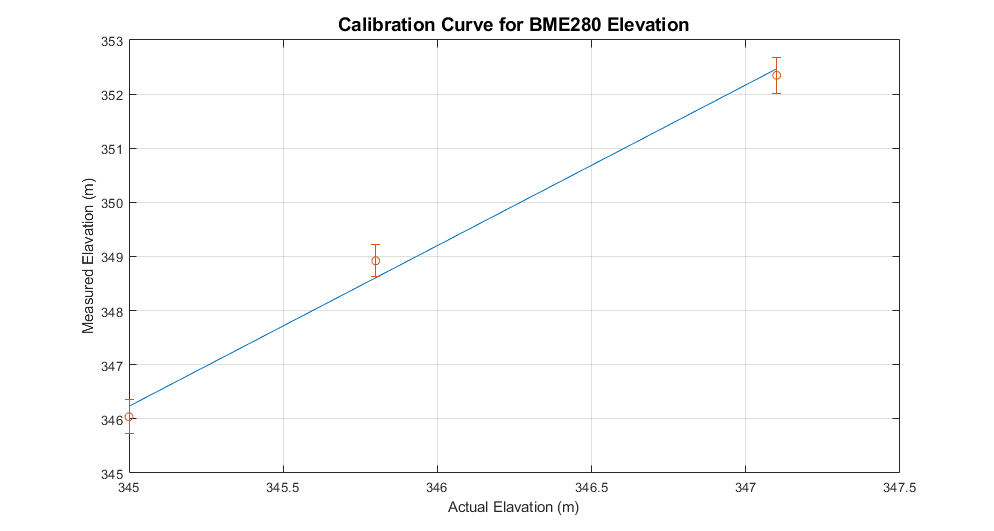
\includegraphics[height=3.2in]{pics/ela_cal.png}}
\caption{Calibration curve for BME280 elevation.}
\label{fig:ela_cal}
\end{figure}

Once again, the percentage error for the elevation readings of the sensor is calculated using Equation 2 and tabulated in Table \ref{table:per_err_e} below.

	\begin{table}[ht]
    \caption{Percentage error for BME280 at various elevations.}
	\vspace{3mm}
	\centering
	\begin{tabular}{cccc}
	\hline
		Measured Elevation & Actual Elevation & Difference & Percentage Error\\
	\hline
		346.04m & 345.00m & 1.04 & 0.30\%\\
		348.92m & 345.80m & 4.12 & 1.19\%\\
		352.48m & 347.10m & 5.38 & 1.55\%\\
	\hline
	\end{tabular}
	\label{table:per_err_e}
	\end{table}

\section{Discussion}
\subsection{Static vs. Dynamic Data Acquisition}
Static and dynamic data acquisition was performed with the BME sensor when collecting temperature data. The static data collection can be seen in Figure \ref{fig:temp_cal}, along with the errors at each point collected in Table \ref{table:per_err}. When looking at Table \ref{table:per_err}, it can be seen that there is a relatively linear error trend for the first three measurements. The error increases as temperature increases, until the last measurement, where the error drops significantly. This may be due to a defect in the temperature sensor which reduces the accuracy up to a certain threshold. In the case of this experiment, it appears to occur somewhere between 26.0\textdegree C and 49.0\textdegree C. This may have occurred because the electrode may have been worn out through extensive use. It may have also experienced corrosion or oxidation, as it is also measuring humidity. \\

The dynamic data collection can be seen in Figure \ref{fig:Subplots} and the performance of dynamic response can observed by analyzing the time constants in Table \ref{table:tau}. It can be noticed that it takes more than twice as long to cool down as opposed to heat up. This may be a result of thermoelectric properties which shows that electrons get excited quicker when heat (energy) is added as opposed to being removed.This phenomena is clearly seen in Table \ref{table:tau}. Another thing to note is that the reference cup for these responses begun at approximately 24\textdegree C. Hence, the difference in temperature from 17\textdegree C is about a 7\textdegree C decrease, and the difference to 37\textdegree C is about a 13\textdegree C increase. Although the temperature increase is just below twice the temperature decrease, the settling time and time constant is more than twice as quick. This shows that the electrodes in the BME sensor are more accustomed to increase temperature increases. \\ 

In order to better see the time constants in the dynamic responses, the sensor should be held for a longer period of time, and wait until a steady state value is reached. The values were displayed on the PuTTY monitor, so the user should wait until the temperature readings remain relatively consistent, indicating that the sensor has reached a steady state value. This should also be done when returning to the reference temperature so that the presence of hysteresis can be better seen.  \\

When looking at Figures \ref{fig:HotCup} and \ref{fig:ColdCup}, it is fairly noticeable that hysteresis is present in the system, and this is inevitable. The sensor represents a first order system which means it may possess thermal capacitance and resistance. This capacitive effect means that it would have memory in the system due to energy storage. The equation representing the first order system corresponds to what is shown below: \\

\begin{equation}
    H(s) = \frac{1}{\tau s+1} \\
\end{equation}
\begin{center}
    \\where $\tau$ = RC
\end{center}

\subsection{Error}
The ultrasonic sensor uses acoustic waves to measure distance. Sound is dependant on the temperature and the pressure of the environment and as such the measurement of the sensor will be dependant on these factors. At a constant pressure of 1atm, the temperature of the system will cause the speed of sound to vary as seen in equation 1. The Conversion factor used in the code for the sensor assumes the surrounding temperature is 25\textdegree C, however the temperature may have varied. The range of the sensor was limited to about 300cm, until the error became very large. The power source for the ultrasonic sensor was 3.3V, which is below the required power rating of the ultrasonic sensor. The output power to generate the ultrasonic pulse wave would be lower which would have affected the range of the sensor. The ultrasonic sensor uses a transducer to detect the incoming wave, however, the transducer may have undergone degradation over time. The transducer could have undergone oxidation and corrosion from previous use. These factors would have impacted the readings of the sensor.\\

The BME280 sensor would have also suffered from errors in the readings as seen in Table 1. The error increases steadily with temperature, then on the last reading it drops to 1.0\%. The change could be due to the composition of the sensor. The sensor uses an electrode to detect humidity and temperature. The electric potential of the electrode varies with respect to the temperature and humidity. The environmental conditions may have caused the electrode to degrade in a similar manner to the transducer in the ultrasonic sensor, in that oxidation and corrosion may have affected it. The errors would have affected the values gathered by the sensor. 

\section{Conclusion}
Overall, this lab analyzed the different functions of an Ultrasonic Distance Sensor and a Breakout Sensor. For the Ultrasonic Distance Sensor, standard deviations were calculated to determine the difference between measured values from the sensor and measured values from a measuring tape. Standard deviations exist due to limitations of the sensor, and all other showed a very good $R^{2}$ value of 0.974, indicating that the sensor displayed accurate measurements. The static responses at 50cm and 300cm show that there was a larger fluctuation in values, the further the distance from the sensor.\\ 

Parameters used for testing the BME Sensor included temperature, altitude, humidity and pressure. This sensor calculated the difference between actual temperature and measured temperature using a thermometer. The calibration curve shows a very good $R^{2}$ value of 0.9842, indicating that the sensor displayed accurate values, however as temperature increased, error increased. The percentage error was calculated and were small values, meaning there were not large sources of error. From the step responses at the different temperatures, time constants were calculated in order to determine the responsiveness of the sensor. From all the step responses at the different parameters, it is also evident that hysteresis was present. Each Sensor used in this lab had different functionalities, but according to our data, the sensors were fairly accurate. 

\section{Future Recommendations}
The procedures in this lab can be improved by modifying some of the techniques used to acquire the data. The BME280 module should be replaced with a sensor that is waterproof. The temperature trials that were done required that the sensor to be dry at all times. For the trials where the temperature of the water had to be recorded, the sensor was placed above the cups. The surrounding temperature fluctuates greatly, and a more accurate and precise reading would have been acquired from the sensor if it were placed directly in water. The readings of the sensor may be improved with this replacement. \\

The temperature of the surrounding area affects the speed of sound, and as a result affects the readings of the ultrasonic sensor. Consequentially, if the temperature of the surroundings was known, then a function in the code could be created that gives the speed of sound at a given temperature. The BME280 sensor to find the temperature can be used alongside the ultrasonic sensor to acquire more reliable results. The temperature would be recorded and processed in the code, which would use equation 1 to determine the speed of sound. The BME280 sensor would need to gather data for the temperature very quickly, so it is suggested that the SPI communication should be implemented. The protocol may use more area than the I\textsuperscript{2}C, however it is faster since it supports a higher bandwidth. These improvements can ensure that the readings for the ultrasonic sensor are more accurate.\\ 

\pagebreak
\begin{thebibliography}{9}

\bibitem{HTM}
HowToMechatronics. (2018). Ultrasonic Sensor HC-SR04 and Arduino Tutorial. [online] Available at: https://howtomechatronics.com/tutorials/arduino/ultrasonic-sensor-hc-sr04/ [Accessed 21 Oct. 2018].

\bibitem{Spark}
Sparkfun.com. (2018). Ultrasonic Sensor - HC-SR04 - SEN-13959 - SparkFun Electronics. [online] Available at: https://www.sparkfun.com/products/13959 [Accessed 21 Oct. 2018].

\bibitem{Prac}
Scherz, P. and Monk, S. (2013). Practical electronics for inventors. 3rd ed. MacGraw-Hill, pp.970 - 973.

\bibitem{Hyper}
Hyperphysics.phy-astr.gsu.edu. (2018). Speed of Sound. [online] Available at: http://hyperphysics.phy-astr.gsu.edu/hbase/Sound/souspe.html [Accessed 21 Oct. 2018].

\bibitem{I2C}
Sparkfun, “I2C”, [Online]. Available: https://learn.sparkfun.com/tutorials/i2c. [Accessed: 21 Oct. 2018].

\bibitem{BME}
Bosch Sensortec, "BME280: Combined humidity and pressure sensor," BST-BME280-DS001-10 Datasheet, Nov. 2015. 

\bibitem{Hub}
Electronics Hub. (2018). Basics of Microcontrollers: History, Structure, Applications. [online] Available at: https://www.electronicshub.org/microcontrollers-basics-structure-applications/ [Accessed 21 Oct. 2018].

\end{thebibliography}

\newpage

\pagenumbering{arabic}% resets `page` counter to 1
\renewcommand*{\thepage}{A\arabic{page}}
\appendix 
\newpage

\section{Appendix}

\subsection{Arduino Scripts}
\lstinputlisting[language=C, style= Matlab-editor, basicstyle = \scriptsize, caption= {us\textunderscore sensor.ino}]{Scripts/us_sensor.ino}
\lstinputlisting[language=C, style= Matlab-editor, basicstyle = \scriptsize, caption= {bme280.ino}]{Scripts/bme280.ino}

\pagebreak
\subsection{MATLAB Scripts}

\lstinputlisting[style= Matlab-editor, basicstyle = \scriptsize, caption= {dist\textunderscore cal.m}]{Scripts/dist_cal.m}
\pagebreak
\lstinputlisting[style= Matlab-editor, basicstyle = \scriptsize, caption= {evetvt.m}]{Scripts/evetvt.m}
\pagebreak
\lstinputlisting[style= Matlab-editor, basicstyle = \scriptsize, caption= {lin\textunderscore reg.m}]{Scripts/lin_reg.m}

\pagebreak
\subsection{Step Responses}
\begin{figure}[!ht]
    \centering
    \makebox[0pt]{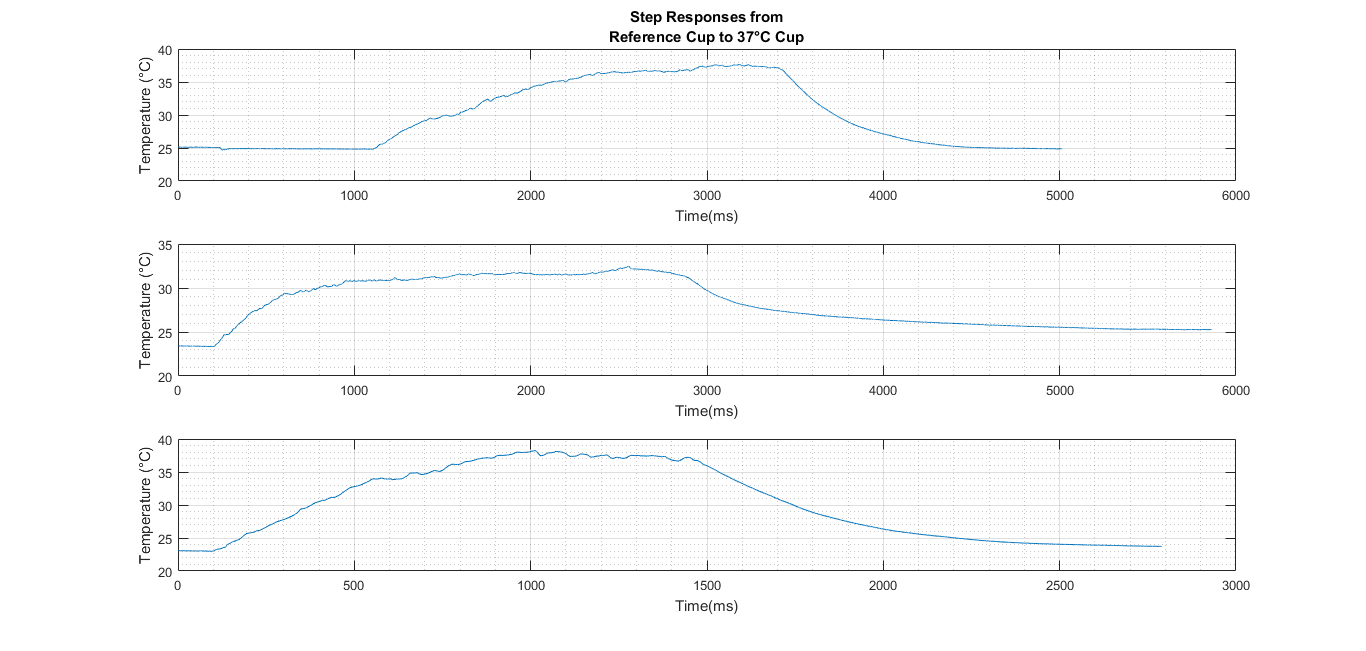
\includegraphics[width=1.2\textwidth]{pics/HotCupStep.png}}
    \caption{Step Responses from Reference Cup to 37\textdegree C Cup}
    \label{fig:HotCup}
\end{figure}

\begin{figure}[!ht]
    \centering
    \makebox[0pt]{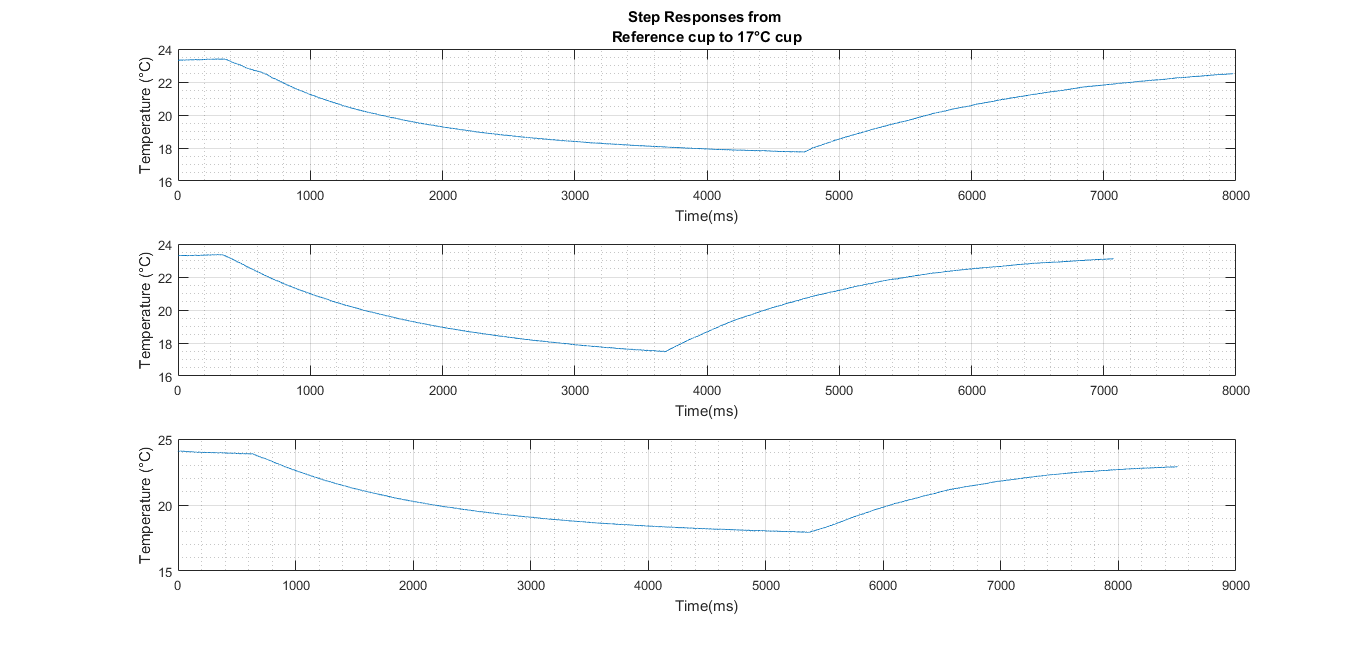
\includegraphics[width=1.2\textwidth]{pics/ColdCupStep.png}}
    \caption{Step Responses from Reference Cup to 17\textdegree C Cup}
    \label{fig:ColdCup}
\end{figure}


\end{document}